%%%%%%%%%%%%%%%%%%%%%%%%%%%%%%%%%%%
\subsection{Gas Analyzers}
\label{sec:fdgen-slow-cryo-gas-anlyz}
% alan h

 Gas analyzers are commercially-produced modules that measure trace quantities of specific gases contained within a stream of carrier gas. The carrier gas for DUNE is argon, and the trace gases of interest are oxygen ($\text{O}_2$), water ($\text{H}_2\text{O}$), and nitrogen ($\text{N}_2$). $\text{O}_2$ and $\text{H}_2\text{O}$ impact the electron lifetime in \dword{lar}, while $\text{N}_2$ impacts the efficiency of scintillation light production. In the \dword{lar} environment, these trace gases represent contaminants that need to be kept at levels below 0.1 ppb.
The Ar is sampled from either the Ar vapor in the ullage or from the \dword{lar} by the use of small diameter tubing run from the sampling point to the gas analyzer. Typically the tubing runs from the sampling points are connected to a switchyard valve that is used to route the sample points to the desired gas analyzers. Fig.~\ref{fig:GA-switchyard} is a photo of such a switchyard.

\begin{dunefigure}[Gas Analyzer switchyard]{fig:GA-switchyard}
  {A Gas Analyzer switchyard that routes sample points to the different gas analyzers.}
  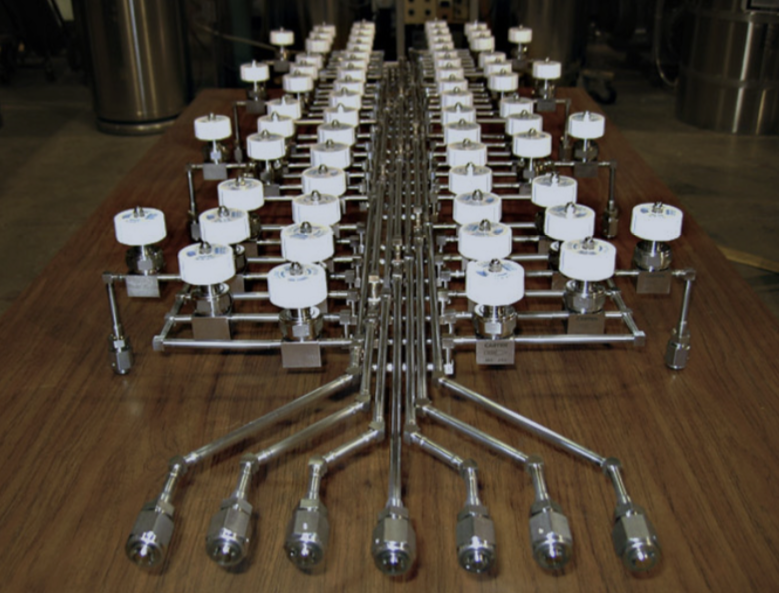
\includegraphics[width=0.35\textwidth]{GasAnalyzerSwitchyard.png}%
\end{dunefigure}

Three examples of usage:

\begin{enumerate}
\item[i)] A proven procedure to eliminate the air atmosphere from the cryostat after detector installation to levels low enough to begin cooldown is an Argon piston purge followed by a recirculation of the remaining argon gas through the filtration system. This process is described more fully in section~\ref{sec:fdgen-slow-cryo-install}. Fig.~\ref{fig:GA-purge} shows the evolution of the $\text{N}_2$, $\text{O}_2$, and $\text{H}_2\text{O}$ levels from gas analyzer data taken during the purge and recirculation stages of the DUNE \num{35}\si{t} Prototype Phase 1 run.

\item[ii)] High precision $\text{O}_2$ and $\text{H}_2\text{O}$ analyzers can track the trace contaminants from the $\>$tens of ppb to the 100s of ppt. This is useful when other means of monitoring the impurity level (e.g., purity monitors, or \dshort{tpc} tracks) are not yet sensitive. Fig.~\ref{fig:GA-O2} shows an example plot of the $\text{O}_2$ level at the beginning of \dword{lar} purification from one of the later \num{35}\si{t} Prototype High Voltage runs.

\item[iii)] The gas analyzers can also monitor the tanker \dword{lar} deliveries purity during the cryostat-filling period. This allows tracking the impurity load on the filtration system and rejecting any deliveries that are out of specifications. Likely specifications for the delivered \dword{lar} are in the $\sim$ten ppm range per contaminant.

\end{enumerate}

\begin{dunefigure}[Gas Analyzer purge]{fig:GA-purge}
  {Plot of the $\text{O}_2$, $\text{H}_2\text{O}$, and $\text{N}_2$ levels during the Piston Purge and Gas Recirculation stages of the \num{35}\si{t} Cryostat Phase 1 run.}
  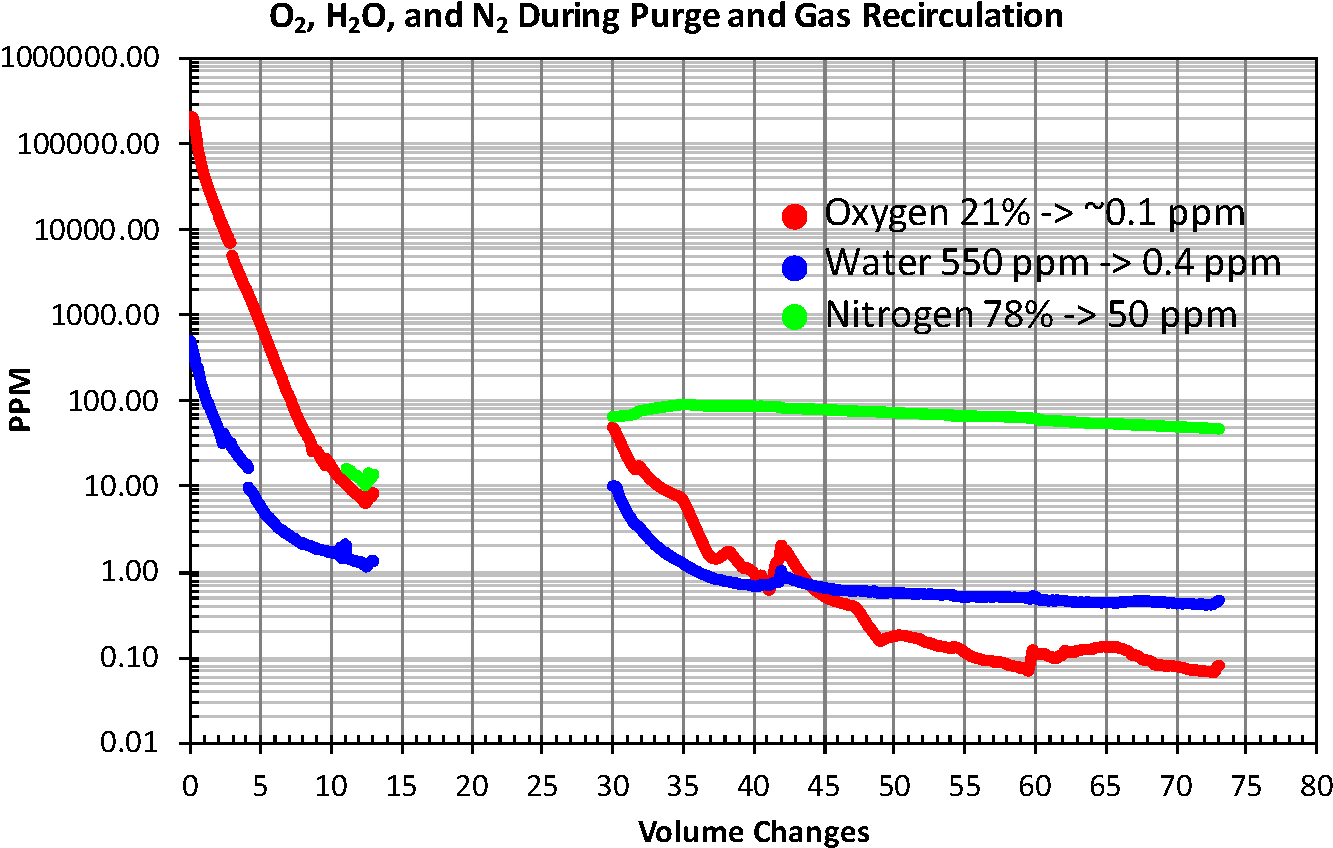
\includegraphics[width=0.65\textwidth]{Phase1_purge_gas_recirculation}%
\end{dunefigure}

\begin{dunefigure}[Gas Analyzer $O_2$ level after \dword{lar} filling]{fig:GA-O2}
  {$\text{O}_2$ as measured by a precision $\text{O}_2$ analyzer just after the 35 ton cryostat was filled with \dword{lar}, continuing with the \dword{lar} pump start and beginning of \dword{lar} recirculation through the filtration system. As the gas analyzer loses sensitivity, the purity monitor is able to pick up the impurity measurement. Note that the purity monitor is sensitive to both $\text{O}_2$ and $\text{H}_2\text{O}$ impurities giving rise to its higher level of impurity.}
  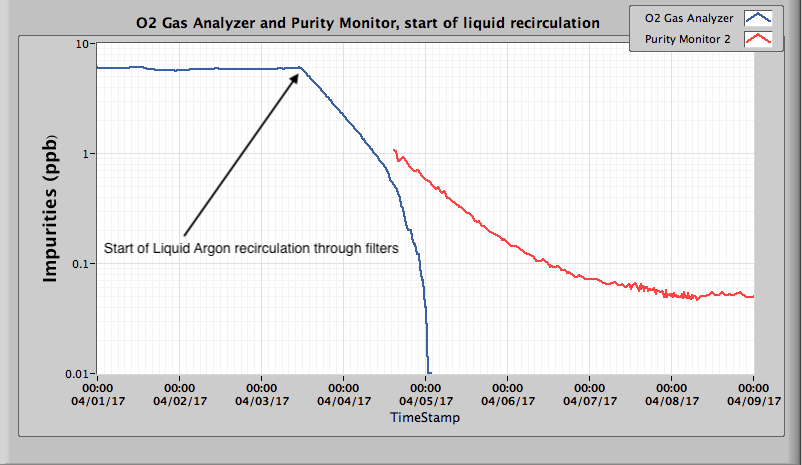
\includegraphics[width=0.7\textwidth]{O2AnalyzerPrM2_HVRun1}% 
\end{dunefigure}

As any one gas analyzer covers only one contaminant species and $\sim$3-4 orders of magnitude of range, multiple units are needed both for the three contaminant gases and to cover the ranges that are seen between the cryostat closure to the beginning of \dshort{tpc} operations:
$\sim \SI{20}{\percent}$ to $\lesssim 100$~ppt for $\text{O}_2$,
$\sim \SI{80}{\percent}$ to $\lesssim 1$~ppm for $\text{N}_2$, and
$\sim \SI{1}{\percent}$ to $\lesssim 1$~ppb for $\text{H}_2\text{O}$.
Since the total cost of these analyzers exceeds $\SI{100}[\textdollar]{k}$, it is useful to be able sample more than a single location or cryostat with the same gas analyzers. At the same time the tubing run lengths from the sample point should be as short as possible in order to keep the response of the gas analyzer timely. This puts some constraints on the sharing of devices since, for example, the argon deliveries are at the surface, perhaps necessitating a separate surface gas analyzer.

